\documentclass{beamer}

\usepackage[UTF8,noindent]{ctexcap}
\usepackage{color}%引入颜色
\usetheme{Berlin}%使用Singapore主题
\usepackage{graphicx}%引入插图
\usepackage{ulem}%删除线
\usepackage{tikz}
\usefonttheme[onlymath]{serif}
\usepackage{minted}%[fragile]
\useoutertheme{infolines}
%\usepackage[orientation=landscape,size=custom,width=16,height=9,scale=0.5,debug]{beamerposter}

\title{图论}
\date{2021年8月20日}
\author{租酥雨}
\begin{document}\small
	
%\usebackgroundtemplate{\tikz\node[inner sep=0pt,opacity=0.3]{\includegraphics[width=16cm,height=9cm]{zsy_background.jpg}};}
	\begin{frame}
	\titlepage
		\begin{center}
		
\includegraphics[width=2.0cm]{zsy.jpg}
		\end{center}
	\end{frame}

\begin{frame}{outline}
	\begin{itemize}
		\item 最小生成树
		\item 最短路
		\item Tarjan
		\item 二分图
		\item 三元环计数
		\item 欧拉回路
	\end{itemize}
\end{frame}
\section{最小生成树}
\begin{frame}{最小生成树}
	最小生成树就是一张图的边权和最小的生成树。\\
	
	所有极小生成树都是最小生成树,这里的极小指的是无法通过更换一条边(从生成树中删去一条边,再加入一条边)使树边权值和变小。\\
	
	所以最小生成树也可以最小化“图中某两点$u, v$间任意路径上的最大边权”,我们把这类的模型称为“货车运输”(NOIP 2013)。\\
	
	最小生成树还有一个性质是,对于一张图的所有最小生成树(可能有多棵)来说,它们同种边权的边的数量是一定的,且在只考虑边权不超过某个阈值$T$的所有边时,任意两点间的连通性是相同的。
\end{frame}
\begin{frame}{求最小生成树的算法}
	Prim:从$1$号点出发,对每个未标记点维护所有已标记点连向它的最小边权,每次找一个最小边权最小的未标记点连边,设之为已标记,并更新其他未标记点的最小边权。可使用堆优化得到$O(m\log m)$的复杂度。\\
	
	Kruskal:边按边权从小到大排序,依次判断能连就连,需要使用并查集维护。时间复杂度为$O(m\log m)$。\\
	
	Borüvka:维护图中的连通块,每轮对每个连通块找出连向外的最小边权的边,尝试把这些边加入最小生成树,如此操作,在每一轮后连通块数量至少减半。时间复杂度为$O(nk\log n)$,其中$k$为“对每个点找连向所在连通块外的最小边权的边”的复杂度。
	
	这种算法一般用于求解(隐式给出的)完全图的最小生成树。
\end{frame}
\subsection{NOIP2013 货车运输}
\begin{frame}{NOIP2013 货车运输}
	\begin{block}{description}
		A 国有 $n$ 座城市,城市之间有 $m$ 条双向道路。每一条道路对车辆都有重量限制,简称限重。
		
		现在有 $q$ 辆货车在运输货物,第 $i$ 辆货车需要从$x$城市运货到$y$城市,问在不超过车辆限重的情况下,最多能运多重的货物。
		
	\end{block}
	\begin{block}{constraint}
		$n, m, q \le 10^5.$
	\end{block}
\end{frame}
\begin{frame}{NOIP2013 货车运输}
	\begin{block}{tutorial}
		问题的关键在于“最大化图中两点间任意路径上的边权最小值”。\\
		
		所以建立一棵最大生成树后,直接查询树上路径最小值即可。
	\end{block}
\end{frame}


\subsection{CodeForces891C Envy}
\begin{frame}{CodeForces891C Envy}
	\begin{block}{description}
		一张$n$个点$m$条边的带权无向图,有$q$次询问,每次询问给出$k_i$条图中的边,问这$k_i$条边能否同时在一棵最小生成树里。
	\end{block}
	\begin{block}{constraint}
		$n, m, q, \sum k_i \le 5 \times 10^5.$
	\end{block}
\end{frame}
\begin{frame}{CodeForces891C Envy}
	\begin{block}{tutorial}
		一次询问中,不同边权的边之间是不会互相影响的,所以只需要判断询问的每种边权的边能不能在出现在同一棵最小生成树里即可。\\
		
		只需要得到Kruskal算法在加入这一种边权的所有边之前维护的并查集结构,就可以判断这些边能否共存。\\
		
		离线处理所有询问,即可方便地维护上述的并查集结构。
	\end{block}
\end{frame}


\subsection{JOISC2014 水壶}
\begin{frame}{JOISC2014 水壶}
	\begin{block}{description}
		有一张$H \times W$的网格图,每个网格是原野、障碍和建筑中的一种。建筑有恰好$P$栋。
		
		原野上很热,每在原野上行进一单位距离就需要一升水,而原野上又没有任何补水的地方,因此必须携带水壶来供水。任何建筑内都可以补满水。
		
		有$Q$个询问,第$i$个询问是问欲从建筑$S_i$走到建筑$T_i$,至少需要多大容积的水壶。
		\begin{center}
			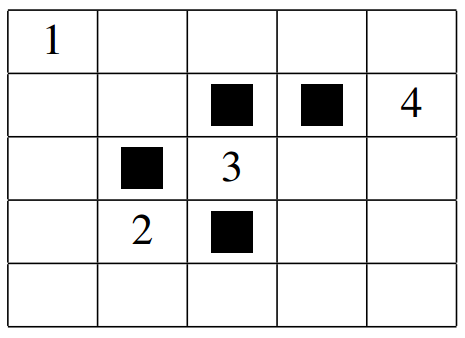
\includegraphics[width=3.0cm]{joisc2014.png}
		\end{center}
	\end{block}
	\begin{block}{constraint}
		$H, W \le 2000, P, Q \le 2 \times 10^5.$
	\end{block}
\end{frame}
\begin{frame}{JOISC2014 水壶}
	\begin{block}{tutorial}
		根据“货车运输”,我们只要对$P$栋建筑求一棵最小生成树就能回答询问了。\\
		
		问题在于怎么建立两两建筑之间的连边。做一个BFS,对每个非障碍的格子求出:离这个格子最近的建筑是哪个以及这个最近距离,当相邻的两个格子的最近建筑不同时,便可以在这两栋建筑之间建立连边。(可以感性地理解为每栋建筑向外扩张势力范围,一旦范围接壤就会产生连边。)\\
		
		可以证明从上述的所有边中就能够建立最小生成树,而这些边的数量是$O(HW)$的,规模在可接受范围内,可以使用Kruskal算法求出最小生成树,其中排序可以采用基数排序。\\
		
		(可能重点在于这种最短路的技巧?)
	\end{block}
\end{frame}


\subsection{NOI2018 归程}
\begin{frame}{NOI2018 归程}
	\begin{block}{description}
		一张$n$点$m$条边的无向图,每条边有具有长度和海拔。
		
		有$q$次询问,每次询问给出起始位置$v$和海拔下限$p$,你在$v$处有一辆车,车只能经过所有海拔不低于$p$的边,你可以选择把车停在任意位置,然后下车步行(没有海拔限制)回到$1$号点。
		
		要求对于每次询问,最小化步行距离。\textbf{强制在线}。
	\end{block}
	\begin{block}{constraint}
		$n \le 2 \times 10^5, m, q \le 4 \times 10^5.$
	\end{block}
\end{frame}
\begin{frame}{NOI2018 归程}
	\begin{block}{tutorial}
		相当于是求“从$v$出发经过海拔大于等于$p$的边能到达的所有点中,与$1$号点距离的最小值”。先通过一遍最短路求出每个点到$1$号点的距离$dis_i$。\\
		
		介绍一下Kruskal重构树,其主要思想就是对Kruskal算法中并查集的连边过程显式地建立出树结构,这样上述“从$v$出发经过海拔大于等于$p$的边能到达的所有点中”就对应并查集连边过程中某个时刻出现的一个连通块,这在Kruskal重构树上恰好对应一棵子树。\\
		
		因此只需要通过二分来定位子树,并维护子树内$dis_i$的最小值即可。
	\end{block}
\end{frame}



\subsection{例题:位运算最优生成树}
\begin{frame}{例题:位运算最优生成树}
	\begin{block}{description}
		给出$n$个数$\{a_i\}_{i=1}^{n}$,建立一张完全图,边$(i, j)$的边权是$a_i \oplus a_j$,其中$\oplus$是任意一个满足交换律的位运算(通过每一位上的真值表来给出)。
		
		求这张图的$\mathrm{optimal = \{maximal, minimal\}}$生成树。
	\end{block}
	\begin{block}{constraint}
		$n \le 10^5, 0 \le a_i < 2^{18}.$
	\end{block}
	\begin{block}{derivatives}
		$\oplus = \mathrm{bitwise\ xor}, \mathrm{optimal = minimal} \Rightarrow $ CodeForces888G Xor-MST
		
		$\oplus = \mathrm{bitwise\ and}, \mathrm{optimal = maximal} \Rightarrow $ Uoj176 新年的繁荣
	\end{block}
\end{frame}
\begin{frame}{例题:位运算最优生成树}
	\begin{block}{tutorial}
		(部分衍生问题存在复杂度更优的解法。)\\
		
		考虑一种统一的做法,考虑使用Borüvka算法。我们每轮需要做的事情是对每个$a_i$,找到一个异色的(不在同一个连通块内)$j$来最大/小化$a_i \oplus a_j$。\\
		
		位运算可以贪心,按照二进制位从高到低,我们每次希望当前的最高位能(填$1$/填$0$/填什么都行)。建立一棵Trie树,这样“填$1$/填$0$”只需要向特定的一边递归即可,而“填什么都行”就比较麻烦,需要预先处理一个Trie树合并,从而让往一边递归实际上起到了往两边递归的效果。\\
		
		需要注意的是Trie树每个节点上需要维护其子树内的两种不同颜色(因为要找且仅要找异色)。该算法的时间复杂度为$O(n\log n\log a_i)$。
	\end{block}
\end{frame}

\section{最短路}
\begin{frame}{最短路}
	BFS:解决所有边权都相同的问题,复杂度$O(m)$。\\
	
	Floyed:复杂度$O(n^3)$,需要注意的是三层循环的枚举顺序,以及当最外层循环变量\texttt{k}枚举到$k$时,数组中\texttt{dis[i][j]}表示的含义是:从$i$到$j$经过编号不超过$k$的中间节点的最短路。\\
	
	Dijkstra:解决边权非负的问题,可以通过堆优化得到$O(m\log m)$的复杂度。\\
	
	Bellman-Ford:进行$n$轮松弛操作(因为最短路的边数不会超过$n$),复杂度$O(nm)$,可以使用队列优化,但理论复杂度无法变优。
	\begin{itemize}
		\item 当使用(队列优化的)Bellman-Ford算法判负环时,正确的做法是记录最短路经过的边数,当边数大于$n$时便说明找到了负环。
	\end{itemize}
\end{frame}
\begin{frame}{最短路}
	
	01最短路(所有边边权$\in \{0,1\}$)可以做到$O(m)$。
	\begin{itemize}
		\item 类似 BFS 的过程,遇到$1$边就丢到队列末尾,遇到$0$边就丢到队列开头。
	\end{itemize}
	\pause
	进一步的,所有边边权$\in [0,k]$的最短路问题可以做到$O(km)$。
	\begin{itemize}
		\item 和前者类似,维护$k+1$个队列即可。
	\end{itemize}
	\pause
	更进一步的,$m_1$条边边权$\in [0, k]$,$m_2$条边边权不受限的最短路问题可以做到$O(km_1 + m_2\log m_2)$。	
	
\end{frame}

\begin{frame}{最短路树}
	这其实是非常简单的东西,就是根据最短路的更新关系建出来的一个树形结构。\\
	
	只是希望大家对这玩意儿能有个印象。
	
\end{frame}

\subsection{CERC2012 Farm and Factory}
\begin{frame}{CERC2012 Farm and Factory}
	\begin{block}{description}
		有一张$n$点$m$条边的无向图,你需要新增一个点并向其余的部分点连边(边权可以是任意实数),使得任何其他的点到$1, 2$两个点的最短路都\textbf{可以不经过}这个新点,要求最小化新点到其余每个点的距离之和。
	\end{block}
	\begin{block}{constraint}
		$n \le 10^5, m \le 3 \times 10^5.$
	\end{block}
\end{frame}
\begin{frame}{CERC2012 Farm and Factory}
	\begin{block}{tutorial}
		“任何其他的点到$1, 2$两个点的最短路都\textbf{可以不经过}新点”这个奇怪的限制实际上是限制了新点的加入不会改变原图中$1, 2$两点的最短路。\\
		
		设每个点$i$(自然不包括新点)到$1$的最短路是$f_i$,到$2$的最短路是$g_i$,到新点的最短路是$s_i$,我们可以得到对于每个$i$,都有$pair(f_i, s_i, s_1), pair(g_i, s_i, s_2)$这两个三元对满足三角不等式(即任两者之和不小于第三者)。\\
		
		因为要最小化$\sum s_i$,所以我们令$s_i = \max\{|f_i - s_1|, |g_i - s_2|\}()$一定不会劣。\\
		
		所以我们只需要确定$s_1, s_2$的取值,然后最小化$\sum \max\{|f_i - s_1|, |g_i - s_2|\}$就可以了。这个形式恰好是点$(s_1, s_2)$与点$(f_i, g_i)$的Chebyshev距离,只需要先转成Manhattan距离(这样两维就独立了),然后对两维坐标分别取中位数即可。
	\end{block}
\end{frame}


\subsection{CodeChef Querying on a Grid}
\begin{frame}{CodeChef Querying on a Grid}
	\begin{block}{description}
		一张$M \times N$的格点(不是格子)图,每条边有个非负边权,根据这个边权可以定义两个格点之间的最短路。
		
		有$Q$次如下两种操作:一种操作是给出两个格点,把两点间最短路上的所有格点的点权加上一个数(点权与最短路无关,这种操作保证\textbf{给出的两格点间最短路唯一}),另一种是查询某个格点的权值。
	\end{block}
	\begin{block}{constraint}
		$M \le 3, N, Q \le 10^5.$
	\end{block}
\end{frame}
\begin{frame}{CodeChef Querying on a Grid}
	\begin{block}{tutorial}
		一个显然的性质是对于任何$j \in [y_1, y_2]$,都存在某个$i \in [1, M]$,使得从$(x_1, y_1)$到$(x_2, y_2)$的最短路经过$(i, j)$。\\
		
		考虑分治,以$(i, mid), i \in [1, M]$作为起点求出到整张图的最短路,便可以得到所有跨越$mid$的点对间的最短路,然后左右两侧分别递归。\\
		
		上面求出了最短路的长度,怎么确定出这条路径呢?只需要建立出最短路树,那么这条路径就对应了最短路树上一条经过根(起点)的路径。\\
		
		需要支持的操作是树上的链加法和单点查询,可以差分为单点加法和子树查询,从而可使用树状数组维护。\\
		
		注意修改的时候只在一棵最短路树上做加法操作,而查询时需要在多棵最短路树上查询一个点的权值和。总时间复杂度为$O(M(N+Q)\log^2 N)$。
	\end{block}
\end{frame}

\subsection{BZOJ4289 Tax}
\begin{frame}{BZOJ4289 Tax}
	\begin{block}{description}
		一个 $n$ 个点 $m$ 条边的无向图,每经过一个点,产生的代价是进入和离开这个点的两条边的边权的较大值。
		
		求从起点 $1$ 到点 $n$ 的最小代价和。起点的代价是离开起点的边的边权,终点的代价是进入终点的边的边权。
	\end{block}
	\begin{block}{constraint}
		$n \le 10^5, m \le 2 \times 10^5.$
	\end{block}
\end{frame}
\begin{frame}{BZOJ4289 Tax}
	\begin{block}{tutorial}
		把题目中的边看成点,暴力建图会使边数达到平方级别。\\
		
		将$\max(a,b)$写成$a+\max(b-a,0)$,先直接计算进入时的边的代价,接着如果$b>a$就再加上一些代价。\\
		
		可以采用板书中的方式建图。
	\end{block}
\end{frame}


\subsection{Luogu2371 墨墨的等式}
\begin{frame}{Luogu2371 墨墨的等式}
	\begin{block}{description}
		对于方程$\sum_{i=1}^na_ix_i = b$,求有多少满足$b \in [l,r]$的$b$使方程存在非负整数解。
	\end{block}
	\begin{block}{constraint}
		$n \le 12, 0 \le a_i \le 5 \times 10^5, 1 \le l \le r \le 10^{12}.$
	\end{block}
\end{frame}
\begin{frame}{Luogu2371 墨墨的等式}
	\begin{block}{tutorial}
		选$a_1$作为基,显然若$b$满足条件,则$b+a_1$也满足。\\
		
		记$f_i$表示用$a_2,a_3,...,a_n$能凑出的最小的模$a_1$等于$i$的数,这部分可以使用最短路算法解决。求出了$f_i$后也便不难求出$[l,r]$中合法$b$的数量。\\
		
		这个东西往往被称为同余类最短路问题,17年人尽皆知的$a\times b - a - b$本质上也属于这类问题。
	\end{block}
\end{frame}

\section{Tarjan}
\begin{frame}{Tarjan全家桶}
	一般来说包含求(无向图)点双连通分量、边双连通分量以及(有向图)强连通分量。\\
	
	算法流程大致可以概括为:建立一棵 DFS 树,对每个节点记录访问时间$dfn_i$以及其 DFS 树子树内节点通过\textbf{一条返祖边}能够到达节点的最小$dfn$。注意在无向图中只存在树边和返祖边,有向图中存在树边、返祖边以及横跨边。\\
	
	算法竞赛领域对Tarjan相关算法的考察点一般为:
	
	\begin{itemize}
		\item 点双连通分量 $\to$ 圆方树 $\to$ 相关树上算法
		\item 边双连通分量 $\to$ 树 $\to$ 相关树上算法
		\item 强连通分量 $\to$ DAG $\to$ DAG上动态规划
	\end{itemize}
	
	一个点唯一存在于一个边双或者强连通分量,但可能存在于多个点双连通分量。
	
\end{frame}

\begin{frame}{圆方树}
	圆方树是一种能够表示点双连通关系的树结构。
	
	\begin{center}
		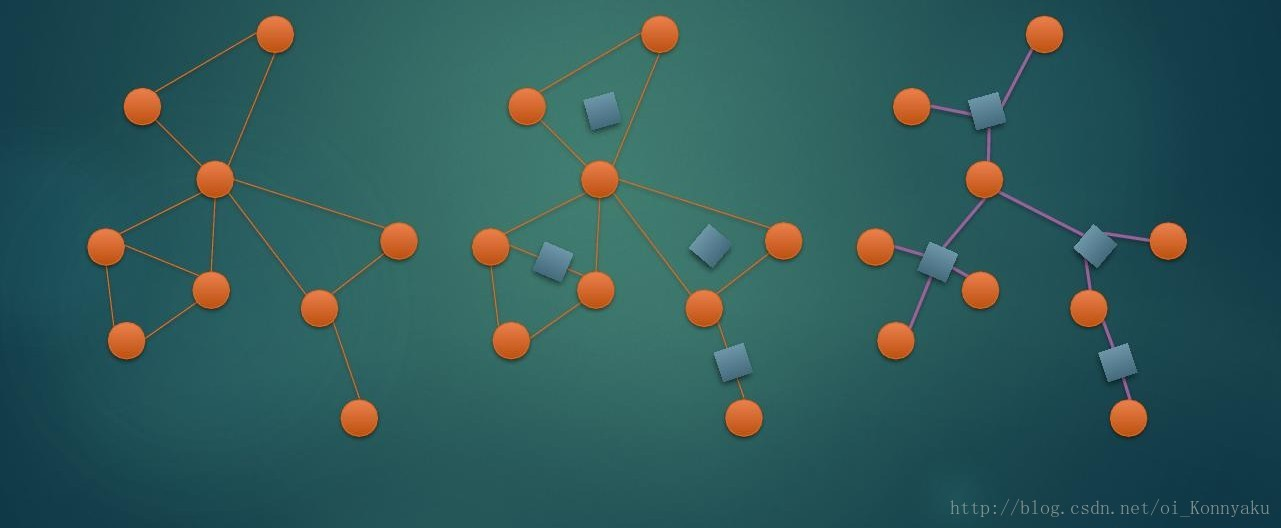
\includegraphics[width=9.0cm]{yuanfangshu.jpg}
	\end{center}

	构建方式为:把原图的中的点看作圆点,对图中的每个点双新建一个方点并向其内部所有圆点连边,随后删除点双中原有的边,只保留一个菊花的结构。\\
	
	如此以来任意两点间路径上的圆点便是割点,或者说必经点。
\end{frame}

\subsection{JSOI2012 越狱老虎桥}
\begin{frame}{JSOI2012 越狱老虎桥}
	\begin{block}{description}
		一张$n$点$m$条边的无向图,边有边权。
		
		Alice会往图中加入一条边,然后Bob会选择割掉图中的一条边使得图不连通(不能割Alice加的那条边)。
		
		Bob希望最小化割掉的边权,Alice希望最大化,求最终被割掉的边权。
	\end{block}
	\begin{block}{constraint}
		$n, m \le 10^6.$
	\end{block}
\end{frame}
\begin{frame}{JSOI2012 越狱老虎桥}
	\begin{block}{tutorial}
		首先边双里的边都不能割,那么把边双缩点,问题被放到了树上。\\
		
		Alice如果选择了加入边$(u, v)$,那么Bob就不能割树上$u, v$路径上的所有边(因为割了之后图还是连通的)。\\
		
		因此按边权从小到大标记树边,直到已标记的树边无法被一条链覆盖为止。无法被覆盖的最后一条边就是答案。
	\end{block}
\end{frame}

\subsection{LOJ2480 One-Way Streets}
\begin{frame}{LOJ2480 One-Way Streets}
	\begin{block}{description}
		有一张$n$点$m$条边的无向连通图,你需要对每一条边定向。有$p$条限制,每条限制形如$x\to y$要求定向后存在从点$x$到点$y$的路径。你需要判断每条边是否可以被唯一定向,若可以,需给出唯一确定的方向。
	\end{block}
	\begin{block}{constraint}
		$n, m, p \le 10^5.$
	\end{block}
\end{frame}
\begin{frame}{LOJ2480 One-Way Streets}
	\begin{block}{tutorial}
		求边双,一个边双连通分量内的所有边的方向都是可任选的。\\
		
		边双缩点变成一棵树,那么问题就变成了树上从一点$x$要走到另一点$y$。树上差分即可。
	\end{block}
\end{frame}

\subsection{UOJ30 Tourists}
\begin{frame}{UOJ30 Tourists}
	\begin{block}{description}
		一张$n$点$m$边无向图,每个点有一个点权,$q$次操作,每次操作为修改一个点的点权或者是询问两点$(u,v)$之间\textbf{所有简单路径}中经过的最小点权。
	\end{block}
	\begin{block}{constraint}
		$n, m, q \le 10^5.$
	\end{block}
\end{frame}
\begin{frame}{UOJ30 Tourists}
	\begin{block}{tutorial}
		建出圆方树,在每个方点上维护整个点双的最小点权,那么每次询问就是查询树上路径最小值。\\
		
		但是在有修改的时候,修改一个圆点的点权会导致它所有相邻方点受到影响,从而使复杂度退化。\\
		
		可以采取的解决方法是:方点中维护的信息不包含其父亲圆点,这样修改一个圆点只需要进一步修改其父亲方点,查询时也只需要在路径 LCA 是方点时额外计算一下其父亲圆点即可。
	\end{block}
\end{frame}

\section{二分图}
\subsection{二分图匹配}
\begin{frame}{二分图匹配}
	二分图是一张不存在奇环的无向图。一般我们会对这张无向图进行黑白染色,并自然地把一种颜色的点放在左侧,另一种颜色的边放在右侧。这样图中就只存在横跨左右两侧的边。\\
	
	一个二分图匹配指的是二分图左侧点集某个子集与右侧点集的某个子集间的一个一一对应,满足对应的左右两侧的点之间存在边。最大匹配顾名思义,就是要最大化这个点集的大小。\\
	
	解决二分图最大匹配的常用算法是匈牙利算法,大致思路是从左侧的一个未匹配点出发,从左向右走未匹配边,从右向左走匹配边,如果存在一条路径最终到达一个右侧的未匹配点,显然该路径长为奇数且匹配边与未匹配边交替(后称\textbf{交错路}),因此可以将该路径上所有边的匹配状态取反,即可使匹配数量加$1$。\\
	
	由于单次运行复杂度最坏为$O(m)$,需运行$n$次,故匈牙利算法解决二分图匹配问题的复杂度为$O(nm)$。若使用 dinic 优化的网络流算法解决二分图匹配问题,时间复杂度为$O(m\sqrt n)$,具体可参考《算法导论》。
	
\end{frame}

\begin{frame}{可行点与必经点}
	\begin{block}{可能在最大匹配中的点}
		\pause
		所有有度数的点都可能在最大匹配中。
	\end{block}
	\pause
	\begin{block}{一定在最大匹配中的点}
		\pause
		先求出任意一组最大匹配$S$,那么一定在最大匹配中的点构成的集合就是$S$的子集。
		
		以左侧点为例,一个属于集合$S$的左侧点$x$可能不在最大匹配中当且仅当存在一个不属于集合$S$的左侧点$y$满足$y$到$x$存在一条交替路。右侧点同理。
		
		或者说,建立匹配$S$的残量网络,从源点能到达的$S$中左侧点以及能到达汇点的$S$中右侧点都可能不在最大匹配中。
		
		其他的点都一定在最大匹配中。
	\end{block}
\end{frame}

\begin{frame}{可行边与必经边}
	\begin{block}{可能在最大匹配中的边}
		\pause
		先求出任意一组最大匹配$S$,$S$中的边都可能在最大匹配中。
		
		其余的边需要考虑两种情况:一种是连接已匹配点和未匹配点的边,这种边一定可以换到匹配中;另一种连接两个已匹配点,要使它出现在匹配中需要找出一个\textbf{交错环}。
		
		依然建立残量网络,上述第二种情况等价于连接的两点在同一个强连通分量中(其实第一种情况也满足)。
	\end{block}
	\pause
	\begin{block}{一定在最大匹配中的边}
		\pause
		依旧是求出任意一组最大匹配$S$,答案是$S$的子集。
		
		从源点能到达的匹配边和能到达汇点的匹配边都可能不在最大匹配中。这是匹配点变更造成的影响。
		
		还需要考虑交替环的影响。连接两端点在同一个强连通分量中的匹配边也可能不在最大匹配中。
	\end{block}
\end{frame}
\subsection{TJOI/HEOI2016 游戏}
\begin{frame}{TJOI/HEOI2016 游戏}
	\begin{block}{description}
		一张$n \times m$的网格图,每个格子都是空地、墙壁或是草丛中的一种。
		
		你可以选择在空地上安放炸弹,炸弹的爆炸范围是从安放炸弹的格子出发向上下左右四个方向延伸直至碰到墙壁或者离开网格图(注意草丛是可以被炸弹穿过的)。
		
		问最多可以安放多少炸弹,使得任意两个炸弹不会互相炸到。
	\end{block}
	\begin{block}{constraint}
		$n, m \le 50, \mbox{墙壁数量}\le 300.$
	\end{block}
\end{frame}
\begin{frame}{TJOI/HEOI2016 游戏}
	\begin{block}{tutorial}
		一行或一列连续的空地/草丛中只能放置至多一个炸弹。\\
		
		题意可以抽象成:选尽量多的空地(放置炸弹),满足这些空地两两不在同一个行或列的连续段中。\\
		
		把行连续段看成二分图一侧的点,列连续段看成二分图另一侧的点,空地看成连接两者的边,便转化成了二分图最大匹配问题。
	\end{block}
\end{frame}
\iffalse
\subsection{Hall 定理}
\begin{frame}{Hall 定理}
	对于一张二分图,设其左侧点集为$V_1$,右侧点集为$V_2$,$|V_1| \le |V_2|$,那么这张二分图有完备匹配(匹配数为$|V_1|$)的充分必要条件是,$V_1$中的任意$k(k = 1, 2, \cdots, |V_1|)$个点与$V_2$中至少$k$个点相邻。\\
	
	上述结论就是Hall定理。它的必要性是显然的,充分性证明可以考虑反正,假设这张二分图的最大匹配非完备,就存在一个左侧的未匹配点$v_x$,记
	\begin{align*}
		S = \{v | v \in V_1\mbox{且在某条从}v_x\mbox{出发的交错路径上}\}\\
		T = \{v | v \in V_2\mbox{且在某条从}v_x\mbox{出发的交错路径上}\}\\
	\end{align*}
	通过证明$|S| = |T| + 1$,且$S$在$V_2$中的相邻点集恰好是$T$,来导出与假设条件的矛盾。\\
	
	Hall 定理在OI中的使用方式往往是通过题目条件把“任意子集”的限制弱化为“任意连续区间”(证明若选取的子集不连续则一定不最劣),从而可以用一些数据结构来维护这个东西。
\end{frame}

\subsection{300iq Contest 1 Dates}
\begin{frame}{300iq Contest 1 Dates}
	\begin{block}{description}
		这道题需要一个主人公,我们不妨管他叫小X。
		
		在接下来的$m$天时间里,有$n$个女孩子想要和小X约会。第$i$个女孩子想要在$[l_i,r_i]$中的某一天和小X约会,且约会后小X会得到$p_i$的愉悦值。
		
		在这里,我们保证$l_i\le l_{i+1}, r_i \le r_{i+1}$。
		
		小X在第$i$天至多和$a_i$个女孩子约会,他希望你帮他求出他能获得的最大愉悦值之和。
	\end{block}
	\begin{block}{constraint}
		$n, m \le 3\times 10^5, 0 \le a_i \le n, 1 \le p_i \le 10^9.$
	\end{block}
\end{frame}
\begin{frame}{300iq Contest 1 Dates}
	\begin{block}{tutorial}
		按照$p_i$从大到小依次判断加入这个区间后是否仍存在完美匹配,这种做法的正确性显然。\\
		
		根据Hall定理,判断是否存在完美匹配,需要对$n$个区间的每个子集$S$,检验是否满足$\sum_{i \in S}b_i \le \sum_{\exists i \in S, j \in [l_i, r_i]}a_j$,其中$b_i \in \{0, 1\}$表示第$i$个区间有没有被选。注意到$\{l_i\}, \{r_i\}$的单调性,枚举$S$时只需要枚举$[1, n]$的子区间即可,即枚举$[L, R] \in [1, n]$,限制要求为$\sum_{i=L}^{R}b_i \le \sum_{j=l_L}^{r_R}a_j$。\\
		
		记$sa_i,sb_i$分别为$a_i$和$b_i$的前缀和,于是得到$sb_R-sb_{L-1}\le sa_{r_R}-sa_{l_L-1}$即$sb_R-sa_{r_R}\le sb_{L-1}-sa_{l_L-1}$。再记$c_i=sb_i-sa_{r_i},d_i=sb_{i-1}-sa_{l_i-1}$,限制为$c_R\le d_L$。\\
		
		考虑每次加入一个区间是企图将某一个$b_x$由$0$改为$1$,观察发现只会有$c_{x...n}$与$d_{1...x}$的大小关系会受到影响,因而维护后缀$c_i$的最大值和前缀$d_i$的最小值判断即可。
	\end{block}
\end{frame}
\fi



\section{无向图三元环计数}
\begin{frame}{无向图三元环计数}
	对一张无向图数有多少无序三元组$(x,y,z)$满足图中存在边$(x,y),(x,z)$以及$(y,z)$。\pause\\
	
	对所有点按度数为第一关键字、标号为第二关键字排序,把所有边按照排序得到的排名重定向(排在前面的指向排在后面的),这样可以保证新生成的有向图是一个DAG,且每个点的出度不超过$\sqrt m$。\\
	
	枚举边$(A,B)$,先遍历$A$的所有出边并标记,再遍历$B$的所有出边,发现一个标记就说明找到了一个三元环。\\
	
	总时间复杂度是$O(m\sqrt m)$,同时也证明了$m$条边的无向图中的三元环数量是$O(m\sqrt m)$级别的。
\end{frame}

\subsection{HDU6144 Counting Stars}
\begin{frame}{HDU6144 Counting Stars}
	\begin{block}{description}
		一张$n$点$m$边无向图,求图中有多少个“A-structure”。
		
		一个“A-structure”被定义为一个有序的节点四元组$(A, B, C, D)$满足边$(A, B), (B, C), (C, D), (A, D), (A, C)$都存在于图中。
	\end{block}
	\begin{block}{constraint}
		$n, m \le 2 \times 10^5.$
	\end{block}
\end{frame}
\begin{frame}{HDU6144 Counting Stars}
	\begin{block}{tutorial}
		一个“A-structure”就是一对有一条边重合的三元环。\\
		
		用前面讲到过的办法数出每条边所处的三元环个数$cnt_i$,$\sum \binom{cnt_i}{2}$就是答案。
	\end{block}
\end{frame}


\section{欧拉回路}
\begin{frame}{欧拉回路}
	俗称一笔画。以下为了方便起见只讨论连通图上的问题。\\
	
	分无向图/有向图两种版本:无向图存在欧拉回路要求所有点的度数均为偶数;有向图则要求所有点入度等于出度。\\
	
	欧拉路不要求回到起点,要求除起点终点外其他点都是偶度点。可以理解为新加一条边连接起点终点后的欧拉回路。\pause\\
	
	多笔画(多条欧拉路)问题?\pause 奇度点两两匹配后求出欧拉回路,把新加的边删除后即得到了多条欧拉路。\pause\\
	
	建议先去 UOJ117 写一份模板,你很可能因此找出代码中藏匿的bug......
	
\end{frame}

\subsection{CodeForces429E Points and Segments}
\begin{frame}{CodeForces429E Points and Segments}
	\begin{block}{description}
		有$n$个闭区间,你需要对每个区间进行黑白染色,使得任意一个点被不同颜色的区间的覆盖次数之差不超过 $1$ 。
	\end{block}
	\begin{block}{constraint}
		$n \le 10^5$,数据保证有解。
	\end{block}
\end{frame}

\begin{frame}{CodeForces429E Points and Segments}
	\begin{block}{tutorial}
		你能猜到这道题目和欧拉回路有关吗?\\
		
		记黑色区间的权值为$1$,白色为$-1$,等价于要求任意一个点被覆盖的所有区间的总权值 $\in [-1,1]$。\\
		
		对于区间$[l,r]$,从$l$向$r+\varepsilon$连一条边,并对所有奇度点按横坐标顺序两两连边(相当于加入了一些新区间),在新生成的图上求出欧拉回路,把从左往右的边染成黑色,从右往左的边染成白色,此时所有点被覆盖区间的总权值均为$0$。\\
		
		注意到新加入的区间集是\textbf{无交}的,因此只要直接去掉这些区间,便可以满足原题中权值$\in[-1,1]$的要求。
		
	\end{block}
\end{frame}

\section{The end}
\begin{frame}
	\begin{center}
		{\huge 谢谢大家!\\  \large 祝大家学业有成!}
	\end{center}
\end{frame}

\end{document}